\section{623 --- Add One Row to Tree}
Given the root of a binary tree, then value $v$ and depth $d$, you need to add a row of nodes with value $v$ at the given depth $d$. The root node is at depth 1.

The adding rule is: given a positive integer depth $d$, for each \textbf{NOT} null tree nodes $N$ in depth $d-1$, create two tree nodes with value $v$ as $N$'s left subtree root and right subtree root. And $N$'s \textbf{original left subtree} should be the left subtree of the new left subtree root, its \textbf{original right subtree} should be the right subtree of the new right subtree root. If depth $d$ is 1 that means there is no depth $d-1$ at all, then create a tree node with value $v$ as the new root of the whole original tree, and the original tree is the new root's left subtree.

\paragraph{Example 1:}
\begin{flushleft}
\textbf{Input:}

A binary tree as following:
\begin{figure}[H]
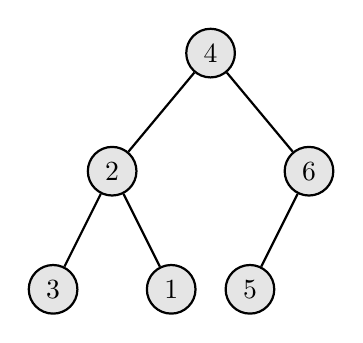
\begin{tikzpicture}
[every node/.style={draw, circle, fill=gray!20!, minimum size=5mm},
level 1/.style={sibling distance=25mm},
level 2/.style={sibling distance=15mm},
thick]
\node{4}
child{node{2} child{node{3}} child{node{1}}}
child{node{6} child{node{5}} child[missing]};
\end{tikzpicture}
\end{figure}

$v = 1$

$d = 2$

\textbf{Output}:
\begin{figure}[H]
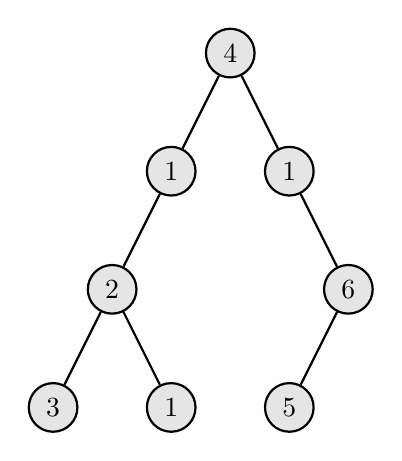
\begin{tikzpicture}
[every node/.style={draw, circle, fill=gray!20!, minimum size=5mm}, thick]
\node{4}
child{node{1} child{node{2} child{node{3}} child{node{1}} } child[missing]}
child{node{1} child[missing] child{node{6} child{node{5}} child[missing]}};
\end{tikzpicture}
\end{figure}

\end{flushleft}
 
%
\paragraph{Example 2:}

\begin{flushleft}

\textbf{Input}:
 
A binary tree as following:

\begin{figure}[H]
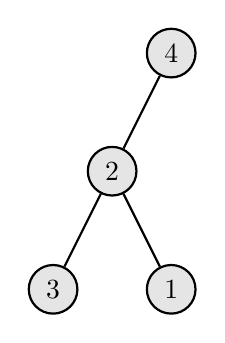
\begin{tikzpicture}
[every node/.style={draw, circle, fill=gray!20!, minimum size=5mm}, , thick]
\node{4}
child{node{2} child{node{3}} child{node{1}}}
child[missing];
\end{tikzpicture}
\end{figure}

$v = 1$

$d = 3$

\textbf{Output}:

\begin{figure}[H]
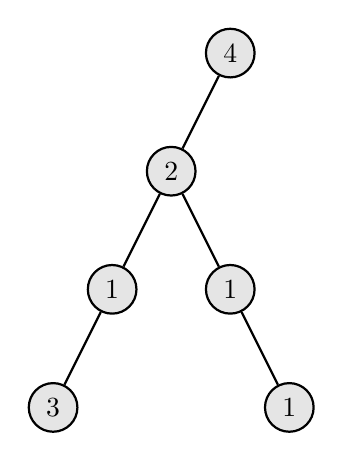
\begin{tikzpicture}
[every node/.style={draw, circle, fill=gray!20!, minimum size=5mm}, thick]
\node{4}
child{node{2} child{node{1} child{node{3}} child[missing]} child{node{1} child[missing] child{node{1}}}}
child[missing];
\end{tikzpicture}
\end{figure}

\end{flushleft}

\paragraph{Note:}

\begin{itemize}
\item The given $d$ is in range [1, maximum depth of the given tree $+ 1$].
\item The given binary tree has at least one tree node.
\end{itemize}

\subsection{DFS With Queue}
\begin{itemize}
\item We can iterate the tree level by level through a queue.
\item When reach depth $d-1$, make changes per the instruction.
\end{itemize}

